 \documentclass[a4paper]{article}
%% Language and font encodings
\usepackage[english]{babel}
\usepackage[utf8x]{inputenc}
\usepackage[T1]{fontenc}

%% Sets page size and margins
\usepackage[letterpaper, portrait, margin=1in,top=1in,bottom=1.5in]{geometry}

%% Useful packages
\usepackage{amsmath}
\usepackage{amssymb}
\usepackage{amsthm}
\usepackage{amsfonts}
\usepackage{mathrsfs}
\usepackage{tikz}
\usepackage{graphicx}
\usepackage[shortlabels]{enumitem}
\newenvironment{exercise}[1]{\textbf{#1.}}

\begin{document}

\begin{flushright}
Cory Glover\\
1/21/20\\
Math 522
\end{flushright}

\begin{center}
HW 3\\
3.10,3.14,3.15,3.16
\end{center}

\begin{exercise}{3.10}
Let $X$ be a node in a graph $\mathscr{G}$ and let $Pa_{X}\mathscr{G}$ be the parents of $X$. Let $P$ be a probaility distribution and $\mathscr{I}(\mathscr{G})$ be the set of global independencies over $P$. Let $Y$ be a non-descendant of $X$. Then $X\perp Y\mid Z$ locally, where $Z\in Pa_X\mathscr{G}$. We prove that $X$ and $Y$ are d-separated. By way of contradiction, assume that $X$ and $Y$ are not d-seperated. Then there exists an active trail between $X$ and $Y$ given $Z$. 

By definition 3.6, this is only possible if for the trail $X\rightleftharpoons X_0\rightleftharpoons X_n\rightleftharpoons Y$ where each $X_i$ is a possible random variable in the trail, then whenever there is a v-structure, $X_{i-1}\rightarrow X_i\leftarrow X_{i+1}$, $X_i$ or one of its descendants is $Z$ and no other nodes are in $Z$. First assume that there are no v-structures. Since $Z$ is a parent of $X$, then $X\rightarrow X_0$. However, since $Y$ is a non-descendant of $X$, then there exists some $X_k\leftarrow X_{k+1}$. That means there must exist at least one v-structure. Thus, $Z$ is in the trail between $X$ and $Y$. This is a contradiction. So assume that there is at least one v-structure. Then $X\leftarrow Z$. This is a contradiction since if $Z$ is in the trail, then all surrounding arrows must point towards $Z$.
So there does not exist an active trail between $X$ and $Y$, hence $X$ and $Y$ are d-separated given $Z$. Since $X,Y$ and $Z$ are general, we see every locally independency is represented in $\mathscr{I}(\mathscr{G})$. So global independencies imply local independencies.
\end{exercise}

%\begin{exercise}{3.11a}
%Let $\mathscr{B}$ be the burglary alarm network from fig 3.15. Consider the marginal distribution $P_\mathscr{B}(B,E,T,N,J,M)$. We construct the diagram
%\begin{center}
%\begin{tikzpicture}[node distance=3cm, thick ]
%\node[draw](B) {Burglary};
%\node[draw](E) [right of = B] {Earthquake};
%\node(S) [below of= B] {};
%\node(S') [below of =E] {};
%\node[draw](T) [left of =S] {TV};
%\node[draw](N) [right of = S'] {Nap};
%\node[draw](J) [below of = S] {JohnCall};
%\node[draw](M) [below of = S'] {MaryCall};
%
%\draw[->](T)--(J);
%\draw[->](N)--(M);
%\draw[->](B)--(E);
%\draw[->](E)--(J);
%\draw[->](E)--(M);
%\end{tikzpicture}
%\end{center}
%\end{exercise}

\begin{exercise}{3.14}
Let $\mathscr{G}$ be the Bayesian network, $X$ the source variable, and $\mathbf{Z}$ be the observations on the network. We want to find all the nodes reachable from $X$ given $\mathbf{Z}$ via active trails. This means we want all the trails from $X$ to $Y$ (where $Y$ is arbitrary) which only have a v-structure $X_{i-1}\rightarrow X_i\leftarrow X_{i+1}$ if $X_i$ or a descendant of $X_i$ is in $Z$. This means there are 3 cases:
\begin{enumerate}
\item $Y$ and $X$ do not have $Z$ in their trail.
\item $Z$ is a descendant of both $X$ and $Y$.
\item $Y$ is $Z$.
\end{enumerate}
We show that the algorithm finds all trails in these three cases.

\begin{enumerate}
\item If $Y$ is an ancestor of $X$, then we look at the trail beginning with $(X,\uparrow)$. We assume that any node on this trail is not in $Z$. We add this to our set $L$ and then select it from $L$, add it to $V$ and add it to $R$ since $X\notin Z$. Since $d=\uparrow$, we add the parents of $X$ to $L$ and repeat, starting with the first parent of $L$. As we continue this, we will pass through all the ancestors of $X$, so we will find the trail between $Y$ and $X$.

If $Y$ is not a direct ancestor of $X$, then after travelling through $X$, we check if $Y$ is a direct ancestor of the new node we select. If it is, we follow the above proof. If it is not, add all the children and all the parents as nodes we could travel to (as to check these active trails connect). Then as we pass through nodes, since $Z$ is not in the trail, we will always continue to check the children and parent trails. Eventually, we will arrive at the node with ancestor $Y$ (or is $Y$). At this point, we will find the trail by visting trails up through the node.
\item Assume that $Z$ is in the trail from $X$ to $Y$. We continue through all possible up and down active trails as in part (i) until we arrive at $Z$. Once we arrive at $Z$, then we know we are travelling down (which must be true because it is a v-structure. We then must travel to the parents of $Z$ (which are in $L$ from phase 1). We then continue the part (i) until we arrive at $Y$. If there is more than one node from $Z$ in the trail, each time we arrive at the node, we know we must travel upwards, which happens in the last if statement of the algorithm. We do this until we have passed through all observed nodes and arrive $Y$.

\item If $Z$ is the node we are travelling to, we can apply part (i).
\end{enumerate}
Hence we can find every trail with this algorithm.
\end{exercise}

\begin{exercise}{3.15}
\begin{enumerate}
\item There is no Bayesian network $I$-equivalent to (a).
\item The graph below is equivalent to (b).
\begin{center}
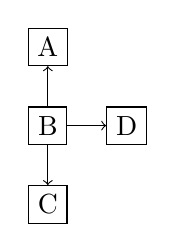
\begin{tikzpicture}
\node[draw](A) {A};
\node[draw](B) [below of=A] {B};
\node[draw](C) [below of=B] {C};
\node[draw](D) [right of=B] {D};

\draw[<-](A)--(B);
\draw[->](B)--(C);
\draw[->](B)--(D);
\end{tikzpicture}
\end{center}
\end{enumerate}
\end{exercise}

\begin{exercise}{3.16}
Let $\mathscr{G}_1$ and $\mathscr{G}_2$ be two graphs over $\mathscr{X}$. Assume that $\mathscr{G}_1$ and $\mathscr{G}_2$ have the same skeleton and v-structures. Let $(X\perp Y\mid Z)$ be a conditional independence in $\mathscr{I}(\mathscr{G}_1)$ given $X$ and $Y$ are d-seperated given $Z$. D-separation means there is not an active trail between $X$ and $Y$ in $\mathscr{G}_1$. This means that there is an observation in the trail between $X$ and $Y$ that is not the center node (or descendant of one) of a v-structure of $\mathscr{G}_1$. Since all the v-structures are the same in $\mathscr{G}_2$, we know that the center node of any v-structure in the trail between $X$ and $Y$ in $\mathscr{G}_2$ is not an observation. Further, neither is one of the descendants, because if it was, it would create a v-structure in $\mathscr{G}_2$ that is not in $\mathscr{G}_1$. However, since the skeleton of $\mathscr{G}_1$ and $\mathscr{G}_2$ are the same, there does exist an observation on the trail between $X$ and $Y$ in $\mathscr{G}_2$. Thus, there does not exist an active trail between $X$ and $Y$ in $\mathscr{G}_2$. So $X$ and $Y$ are d-separated in $\mathscr{G}_2$. Further, since $X\perp Y\mid Z$ in $\mathscr{G}_1$, then must be independent given $Z$ in $\mathscr{G}_2$ since the skeleton is the same and $Z$ must be between $X$ and $Y$ without being in a v-structure. So $(X\perp Y\mid Z)\in\mathscr{I}(\mathscr{G}_2)$. So $\mathscr{I}(\mathscr{G}_1)\subseteq\mathscr{I}(\mathscr{G}_2)$. By the exact same argument, $\mathscr{I}(\mathscr{G}_2)\subseteq\mathscr{I}(\mathscr{G}_1)$. So $\mathscr{I}(\mathscr{G}_1)=\mathscr{I}(\mathscr{G}_2)$.
\end{exercise}
\end{document}